\documentclass[12pt]{article}
\usepackage[utf8]{inputenc}
\usepackage{cite}
\usepackage[spanish]{babel}
\selectlanguage{spanish}
\usepackage{graphicx}
\graphicspath{ {files/} }
\usepackage{url}
\usepackage{natbib}




\title{Reporte sobre la Actividad 5}
\author{García Parra Pedro}
\date{Febrero 2019}

\begin{document}

\maketitle

En esta actividad se pidió analizar algunos de los indices propuestos por un grupo de expertos sobre la detección y monitoreo de índices que miden los efectos del Cambio Climático sobre datos obtenidos del Servicio Meteorológico Nacional de la Comisión Nacional del Agua. En particular elegí los datos sobre Obregón. 

El principal problema para la realización de esta actividad fue la falta de datos y los datos "Nulos" o símplemente datos que no cumplen con los requisitos del índice.
Para lidiar con los datos "Nulos" primero tenemos que decirle a la libreria de pandas que cuando lea los datos ignore los "Nulos".

El problema con los datos que no cumplen con los requisitos del índice fue un poco más complicado de resolver y las soluciones varian dependiendo del índice.
Por ejemplo, para el índice 4 (Longitud de la estación de cultivo por año); mis datos no tenian ningun sólo dato que cumpliera con esa condición (Periodo entre los primeros 6 días seguidos del año  Tprom $>$ 5ºC, y los últimos 6 días seguidos del año con Tprom $<$ 5ºC) por lo que tuve que hacer que el codigo reconociera los datos cuando un dato sirve y cuando no, y cuando no sirviera que tratara ese valor como un valor "N/A" (No disponible). Pero debido a que ninguno de mis datos cumple con la condición, la grágica quedó vacía, como se muestra en la figura(\ref{fig:indice4}). Pero gracias a que hice ésto, el codigo funciona para cualquier tabla de datos (aunque funciona muy lento para tablas con muchos datos).

Con el analisis realizado en ésta actividad se puede apreciar un cambio en la temperatura de obregon. Podemos ver para los años de 1990 al2011 la temperatura iba en aumento figura(\ref{fig:indice5}). Pero por falta de datos no se pudo realizar un analisis sobre los últimos 8 años para poder apreciar bien este aumento de la temperatura.

 Tambien podemos ver, en la figura(\ref{fig:indice2}), que casi todos los días de todos los años puen ser considerados dias de verano donde la temperatura es mayor a 25ºC, además el numero de éstos días ha aumentado con el paso de los años.
 
 Con respecto a las lluvias, podemos ver en la figura(\ref{fig:indice15}) que el periodo entre lluvias es muy largo, incluso podemos apreciar que ha habido años donde el maximo del periodo de sequía ha durado casi dos meses. Esta tendencia a periodos largos entre lluvias no se ve afectada mucho con el paso de los años, quizá podemos ver que las temporadas de sequía tienden a ser más cortas.
 
 En general se puede observar que es un lugar calido seco, con pocas precipitaciones anuales y periodos de sequía altos. Además, durante los años la temperatura ha aumentado, mientras que la cantidad de precipitación anual se mantiene mas o menos igual a lo largo de todos los datos.
 
 \begin{figure}
    \centering
    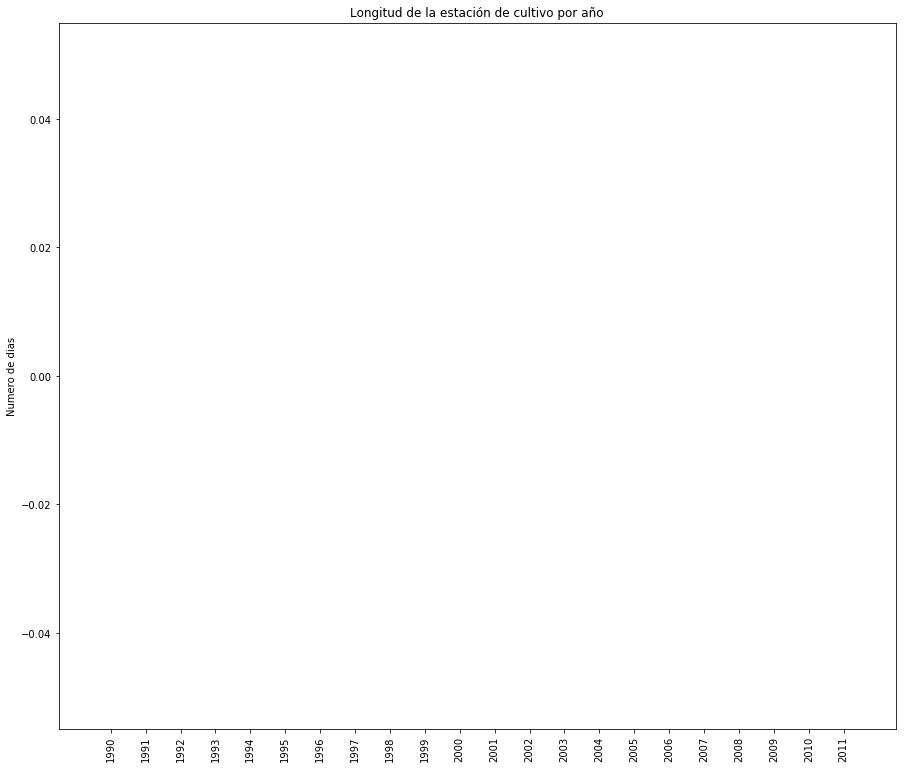
\includegraphics[scale= .25]{indice4.png}
    \caption{Gráfica que representa la longitud de la temporada de cosecha}
    \label{fig:indice4}
\end{figure}
\begin{figure}
    \centering
    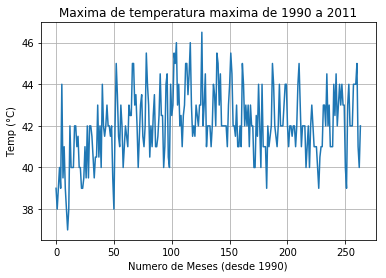
\includegraphics[scale=.8]{indice5.png}
    \caption{Gráfica que representa la maxima de la temperatura mensual}
    \label{fig:indice5}
\end{figure}
\begin{figure}
    \centering
    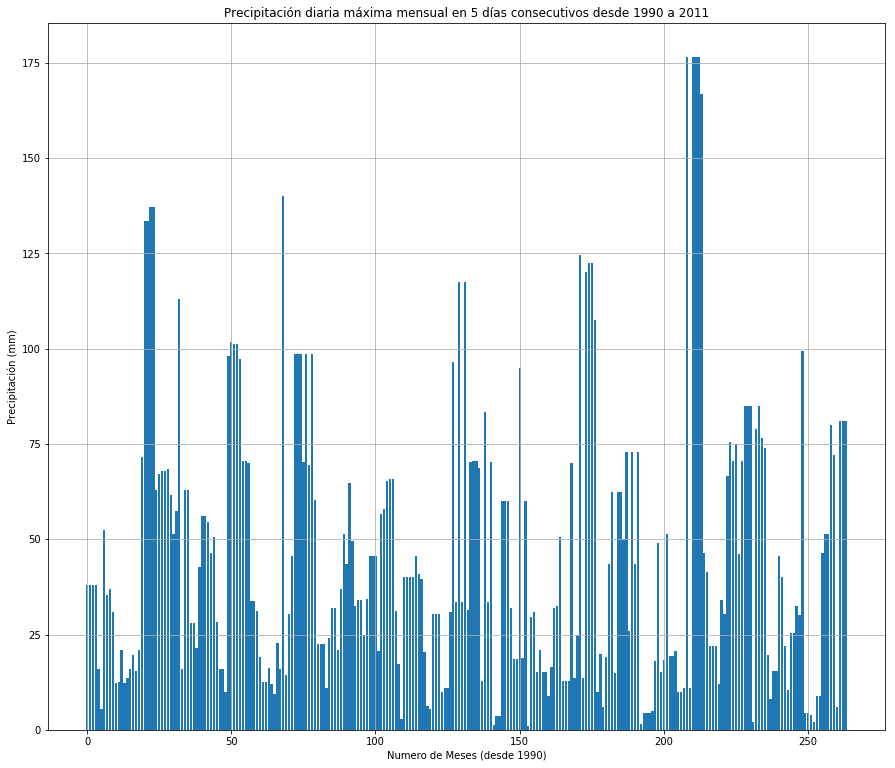
\includegraphics[scale=.3]{indice11.png}
    \caption{Gráfica que representa el maximo de precipitacion en 5 dias seguidos durante todos los años}
    \label{fig:indice11}
\end{figure}
\begin{figure}
    \centering
    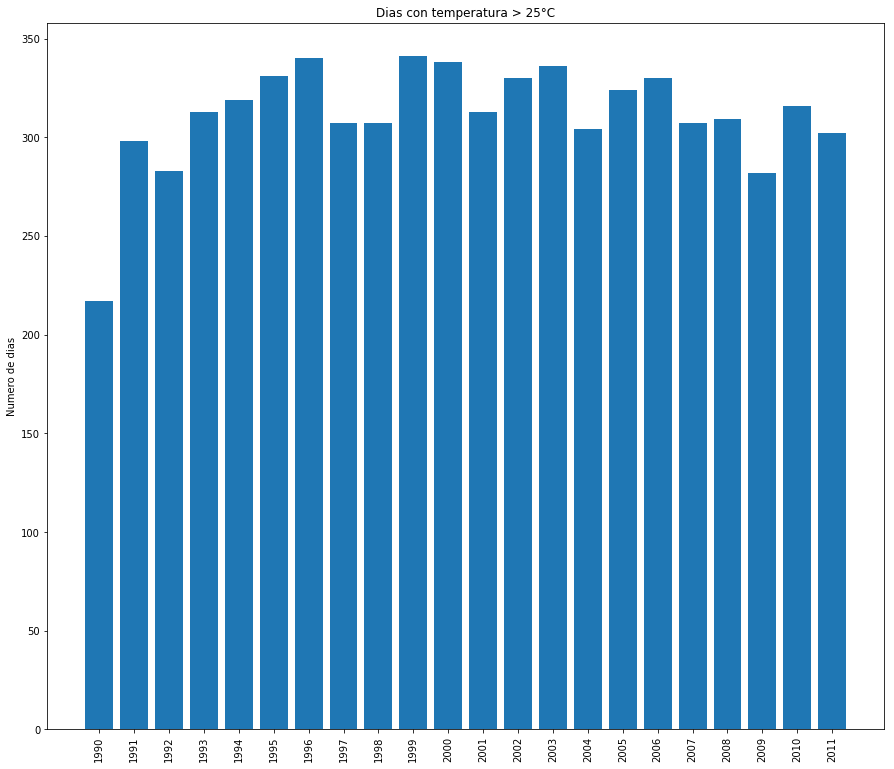
\includegraphics[scale=.3]{indice2.png}
    \caption{Gráfica que representa la cantidad anual de días con temepratura mayor a 25ºC}
    \label{fig:indice2}
\end{figure}
\begin{figure}
    \centering
    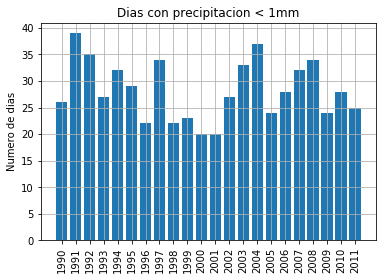
\includegraphics[scale=.8]{indice15.png}
    \caption{Gráfica que representa el numero de dias consecutivos con precipitaciones menores a 1mm}
    \label{fig:indice15}
\end{figure}
\end{document}
